\begin{figure*}[t]
\centering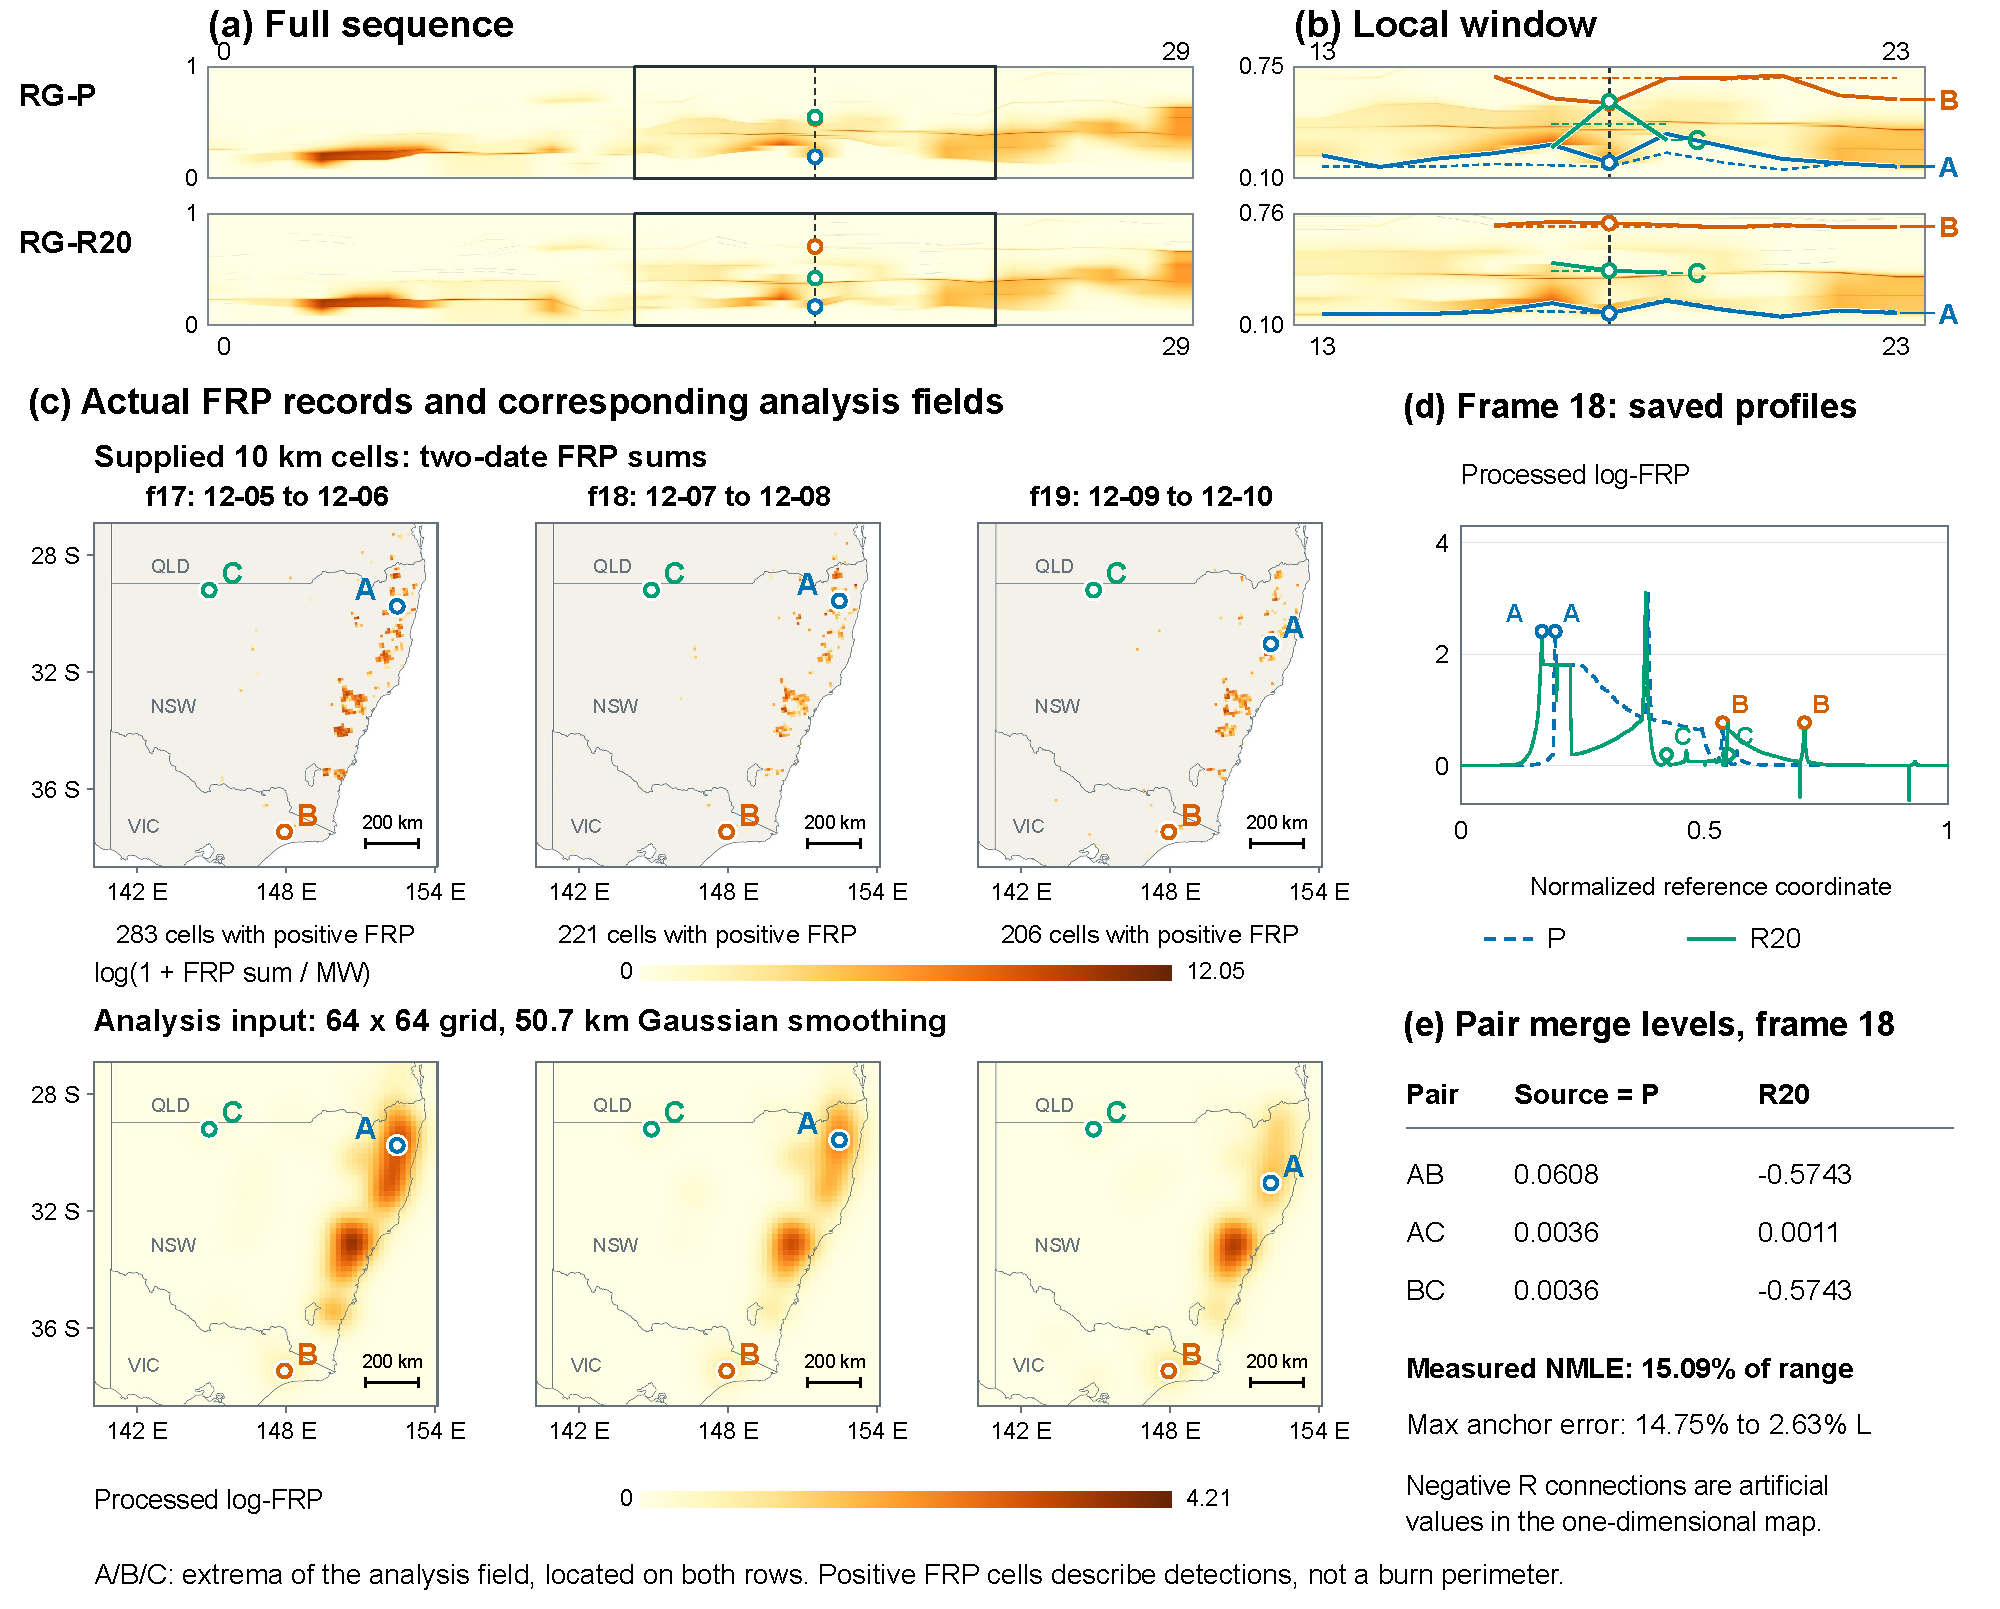
\includegraphics[width=\textwidth]{figures/Fig7.pdf}
\caption{Wildfires: RG-MTM-P/R over all 30 frames (a), with frames 13--23 enlarged (b). Panel (c), top: actual supplied 10-km FRP cell polygons for December 5--6, 7--8, and 9--10, 2019 (frames 17--19), on a geographic basemap~\cite{NaturalEarth:WildfireAdmin1}. Only cells with positive two-date FRP sums are colored; they indicate recorded fire activity rather than a burn perimeter. Bottom: the corresponding saved analysis fields, after aggregation onto a $64\times64$ grid (20.3-km cells), $\log(1+\mathrm{FRP}/\mathrm{MW})$, 50.7-km Gaussian smoothing, and the declared weak background. Both rows share the same extent, with geographic coordinates and 200-km scale bars. Tracks $A=3$, $B=48$, $C=52$ mark the same analysis extrema on both rows. Yellow--orange--brown uses fixed ranges 0--12.05 for supplied cells and 0--4.21 for processed fields and maps. Solid traces in (b) are anchors; dashed traces are references. At frame 18, relaxation reduces maximum displacement from 14.75\% to 2.63\% at 15.09\% actual NMLE. Panels (d)--(e) retain complete saved P/R scalar profiles and measured pair connection values. Negative connections are artificial map output, not negative observed FRP. This selected maximum-obstruction witness explains the mechanism; complete-sequence statistics and baseline panels are reported separately (Supplement S10). Temporal colour transitions use display interpolation only; saved frames, anchors, and evaluation samples are unchanged.}
\label{fig:fire_events}
\end{figure*}
